\documentclass[conference]{IEEEtran}
\IEEEoverridecommandlockouts

\usepackage{cite}
\usepackage{amsmath,amssymb,amsfonts}
\usepackage{graphicx}
\usepackage{textcomp}
\usepackage{xcolor}
\usepackage{booktabs}
\usepackage{array}
\usepackage{tikz}
\usetikzlibrary{positioning,arrows.meta,shapes.geometric,fit,backgrounds,calc}
\usepackage{algorithm}
\usepackage{algpseudocode}
\usepackage[hidelinks]{hyperref}

\newcommand{\status}[1]{\textsc{#1}}

\begin{document}
\bstctlcite{IEEEexample:BSTcontrol}

\title{Agentic Pilot: An Evidence-Driven Local Autonomous AI Agent Framework\\for Privacy-Preserving Intelligent Task Automation}

\author{\IEEEauthorblockN{Sudesh P}
\IEEEauthorblockA{\textit{Department of Computing Technologies}\\
\textit{SRM Institute of Science and Technology}\\
Kattankulathur, India\\
sp3782@srmist.edu.in}
\and
\IEEEauthorblockN{Dr. Kanchana M}
\IEEEauthorblockA{\textit{Department of Computing Technologies}\\
\textit{SRM Institute of Science and Technology}\\
Kattankulathur, India\\
kanchanm@srmist.edu.in}}

\maketitle

\begin{abstract}
Browser agents built on language models can report unfinished tasks as done, and many send every screenshot to a hosted model. We present Agentic Pilot, an open-source browser agent that runs its models locally and may report completion only when a rule-based predicate over the observed page holds, storing each decision's inputs as evidence. We formalize evidence-gated completion with false-completion and false-rejection rates and evaluate it at component level in the agent's real verification node. On 42 held-out constructed states frozen before testing, the gate withheld 9 of 22 unsatisfied states (95\% interval 0.23--0.61) and rejected 1 of 20 satisfied ones. It was correct on more states than a dispatch-only rule (exact McNemar $p=0.021$) but not significantly more than an error-check-only detector ($p=0.070$), and below the 20 of 23 it withheld on its design states, because its checks are keyed to request wording. A decision costs a median of 27\,ms and no model call. By default the model client refuses non-loopback endpoints, and in 70 episodes with a scripted stand-in model server the agent's Python processes connected only to 127.0.0.1. Measurements also show that memory retrieval lacks a relevance threshold and recovery misses absent confirmations. A seeded simulation, revised post hoc, indicates that the gate's benefit depends on the unmeasured rate of premature completion claims.
\end{abstract}

\begin{IEEEkeywords}
LLM agents, web agents, local inference, data locality, completion verification, task automation
\end{IEEEkeywords}

\section{Introduction}

Language-model agents now operate software for people: they open pages, fill in forms and read results~\cite{zhou2024webarena,he2024webvoyager,xie2024osworld}. Many send each observation, often a screenshot of a logged-in page, to a hosted multimodal model~\cite{he2024webvoyager,zheng2024seeact,zhang2025ufo}, although such screens carry names, messages and account data, and language models can leak personal information~\cite{lukas2023pii}. An agent can also stop too early. We call this \emph{premature completion}: a terminal ``done'' while the page does not satisfy the goal, for example after opening the search engine but before issuing the query. Each action succeeded; the task did not. In most agents a model decides that the task is finished~\cite{yao2023react,shinn2023reflexion}, and intrinsic self-correction is unreliable~\cite{huang2024cannot}.

We address three gaps. \textbf{G1:} in-loop completion checks over observed state are rarely measured on held-out data. \textbf{G2:} the contribution of each kind of evidence is unknown. \textbf{G3:} locality claims of ``local'' agents are rarely tested.

Agentic Pilot acts in a Chromium browser. It is autonomous in that it plans and executes actions without step-by-step instructions; the user approves high-risk tasks and solves CAPTCHAs. It is privacy-preserving in a narrow sense: by default its model client sends prompts and screenshots only to a model server on the loopback interface, and it stores task records, memory and evidence only in local files. Our contributions are:
\begin{enumerate}
\item a formulation of evidence-gated completion that separates action dispatch from task completion, with false-completion and false-rejection rates;
\item measured (\status{actual}) error rates of the gate on 92 constructed states in three sets, one frozen before testing, with intervals, paired tests and a per-conjunct ablation;
\item loopback-only endpoint enforcement with an egress test, and measurements exposing failure modes of memory and recovery; and
\item an open-source implementation, a seeded simulation (\status{synthetic}) with every assumption stated, and an end-to-end harness for task-level studies.
\end{enumerate}

\section{Related Work}

\textbf{Agents.} ReAct interleaves reasoning with tool actions~\cite{yao2023react}; Reflexion and RCI let the model critique its own attempts~\cite{shinn2023reflexion,kim2023rci}. Mind2Web, WebVoyager and SeeAct act on web pages from DOM or screenshots~\cite{deng2023mind2web,he2024webvoyager,zheng2024seeact}; WebArena and OSWorld evaluate agents with functional checks after the episode~\cite{zhou2024webarena,xie2024osworld}; UFO and AppAgent control desktop and mobile applications~\cite{zhang2025ufo,zhang2025appagent}. These works say little about when the agent itself may conclude that a task is done.

\textbf{Completion checking.} WebVoyager evaluates trajectories with a multimodal judge~\cite{he2024webvoyager}, Pan et al.\ use model-based evaluators~\cite{pan2024autonomous}, and Sumyk and Kosovan evaluate a vision-language completion judge~\cite{sumyk2025done}. Our gate applies execution monitoring from planning and robotics~\cite{fikes1972planex,pettersson2005execution} to an LLM agent's completion claims inside the loop.

\textbf{Memory, security and local models.} Retrieval-augmented memory~\cite{lewis2020rag,packer2023memgpt} supports agents; indirect prompt injection threatens them~\cite{greshake2023indirect,debenedetti2024agentdojo}. Open-weight models such as Qwen2.5~\cite{yang2024qwen25} with quantization~\cite{lin2024awq} run on consumer hardware. Table~\ref{tab:related} compares representative systems.

\begin{table}[!t]
\centering
\caption{Comparison with representative systems, from what each paper reports. Env.: W live websites, Wr self-hosted or cached pages, Ws simulated web, tool or text environment, D desktop OS, Mo mobile. Exec.: A agent, B benchmark, M model. Completion: who decides that a task is done. Evid.: per-step state artifacts. Mem.: memory across steps or episodes. Deploy.: L open-weight models, H hosted only. Eval.: E2E end-to-end tasks, Off offline step prediction, C+S component tests and simulation. Y yes, P partial, N no, n.r.\ not reported. All listed systems released code.}
\label{tab:related}
\setlength{\tabcolsep}{1.7pt}
\scriptsize
\begin{tabular}{@{}lllllccc@{}}
\toprule
System & Env. & Exec. & Completion & Evid. & Mem. & Deploy. & Eval. \\
\midrule
ReAct~\cite{yao2023react}               & Ws & A & model & N & N & H & E2E \\
Reflexion~\cite{shinn2023reflexion}     & Ws & A & model$^{a}$ & N & Y & H & E2E \\
WebArena~\cite{zhou2024webarena}        & Wr & B & benchmark & n.r. & N & H & E2E \\
Mind2Web~\cite{deng2023mind2web}        & Wr & B & n/a & P & N & L & Off \\
WebVoyager~\cite{he2024webvoyager}      & W & A & model; judge$^{b}$ & Y & N & H & E2E \\
SeeAct~\cite{zheng2024seeact}           & W, Wr & A & model & n.r. & N & P & E2E, Off \\
OSWorld~\cite{xie2024osworld}           & D & B & benchmark & n.r. & N & L & E2E \\
UFO~\cite{zhang2025ufo}                 & D & A & model & n.r. & P & H & E2E \\
AppAgent~\cite{zhang2025appagent}       & Mo & A & model & n.r. & Y & H & E2E \\
CogAgent~\cite{hong2024cogagent}        & Wr, Mo & M & n/a & N & N & L & Off \\
MemGPT~\cite{packer2023memgpt}          & Ws & A & n/a & N & Y & H & E2E$^{e}$ \\
AgentDojo~\cite{debenedetti2024agentdojo} & Ws & B & benchmark & n.r. & N & L & E2E \\
\midrule
Agentic Pilot (ours)                    & Wr$^{c}$ & A & in-loop rule & Y & P$^{d}$ & L & C+S \\
\bottomrule
\end{tabular}
\vspace{2pt}

\raggedright\scriptsize
$^{a}$An evaluator gives feedback between trials. $^{b}$Used for evaluation. $^{c}$Evaluated only on constructed states and self-hosted sites; the implemented backend targets live websites, and a desktop backend is designed. $^{d}$Implemented; retrieval measured on 10 queries over a synthetic corpus, effect on tasks studied only by simulation. $^{e}$Document QA and conversation tasks, not web tasks.
\end{table}


\section{Problem Formulation}
\label{sec:problem}

The agent observes a state $s_t$ through an observation (URL, title, element list, screenshot). A planner maps a goal $g$, a plan $P$ and the observation to an action $a_t$, whose execution returns a \emph{dispatch flag} $\alpha_t\in\{0,1\}$ that says only that the call returned without error. The agent may report completion only when a predicate holds on the state observed after the action:
\begin{equation}
\Phi(g,s_{t+1},P,\sigma) = \textstyle\bigwedge_{c\in C(g,P)} c(s_{t+1}) \wedge \pi(P) \wedge \neg\beta(s_{t+1},\sigma),
\label{eq:phi}
\end{equation}
where $C(g,P)$ are the postconditions the goal and plan imply, $\pi(P)$ states that no step is pending, and $\beta$ is a blocking condition (a bot-check page, an unapproved high-risk action) with approval state $\sigma$. Dispatch does not imply completion: $\alpha_t=1\not\Rightarrow\Phi=1$.

\textbf{Implemented predicate.} $\Phi$ is the conjunction of: no error URL or title, bot-check page, or unexpected sign-in page ($E$); not still on a search engine's home page when a search, extraction or multi-step plan was requested ($H$); a results page for the quoted query ($Q$); the requested text present in an input ($T$); for extraction requests, an answer mentioning a content word of $g$ ($X$); and no pending plan step ($R$). Each conjunct is instantiated only when its trigger words occur. A pre-check implements $\beta$ and halts the task as \textsc{Blocked}. Fig.~\ref{fig:verify} shows the decision path. $\Phi$ has no tunable threshold, so its trade-off between false completions and false rejections is characterized by removing conjuncts. Every evaluation of $\Phi$ is stored with the observed values it used, so a decision can be audited after the task.

\begin{figure}[t]
\centering
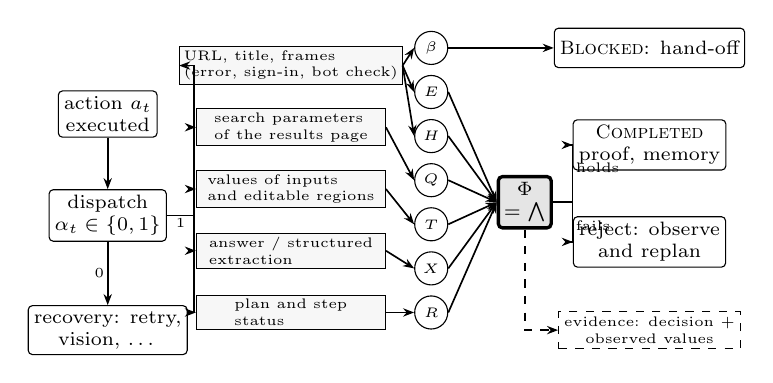
\begin{tikzpicture}[
  x=0.99cm, y=1.12cm,
  font=\scriptsize,
  b/.style={draw, rounded corners=1.5pt, align=center, inner sep=2pt, minimum height=0.5cm, fill=white},
  e/.style={draw, align=left, inner sep=1.5pt, font=\tiny, minimum width=2.4cm, fill=gray!6},
  c/.style={draw, circle, inner sep=0.5pt, minimum size=0.42cm, font=\tiny, fill=white},
  arr/.style={-{Stealth[length=1.4mm]}, semithick},
  lab/.style={font=\tiny, inner sep=1pt}]

\node[b] (act) at (0,0) {action $a_t$\\executed};
\node[b] (alpha) at (0,-1.15) {dispatch\\$\alpha_t\in\{0,1\}$};
\node[b] (rec) at (0,-2.45) {recovery: retry,\\vision, \dots};

\node[e] (ev1) at (2.35, 0.55) {URL, title, frames\\(error, sign-in, bot check)};
\node[e] (ev2) at (2.35,-0.15) {search parameters\\of the results page};
\node[e] (ev3) at (2.35,-0.85) {values of inputs\\and editable regions};
\node[e] (ev4) at (2.35,-1.55) {answer / structured\\extraction};
\node[e] (ev5) at (2.35,-2.25) {plan and step\\status};

\node[c] (cB) at (4.15, 0.75) {$\beta$};
\node[c] (cE) at (4.15, 0.25) {$E$};
\node[c] (cH) at (4.15,-0.25) {$H$};
\node[c] (cQ) at (4.15,-0.75) {$Q$};
\node[c] (cT) at (4.15,-1.25) {$T$};
\node[c] (cX) at (4.15,-1.75) {$X$};
\node[c] (cR) at (4.15,-2.25) {$R$};

\node[b, fill=gray!20, very thick] (and) at (5.35,-1.0) {$\Phi$\\$=\bigwedge$};
\node[b] (ok) at (6.95,-0.35) {\textsc{Completed}\\proof, memory};
\node[b] (no) at (6.95,-1.45) {reject: observe\\and replan};
\node[b] (blk) at (6.95,0.75) {\textsc{Blocked}: hand-off};
\node[draw, dashed, align=center, inner sep=2pt, font=\tiny] (store) at (6.95,-2.45) {evidence: decision +\\observed values};

\draw[arr] (act) -- (alpha);
\draw[arr] (alpha) -- node[lab, left] {0} (rec);
\draw[arr] (alpha.east) -- node[lab, below] {1} ++(0.35,0) |- (ev1.west);
\foreach \n in {ev2,ev3,ev4,ev5} \draw[arr] ($(alpha.east)+(0.35,0)$) |- (\n.west);
\draw[arr] (ev1.east) -- (cB.west); \draw[arr] (ev1.east) -- (cE.west); \draw[arr] (ev1.east) -- (cH.west);
\draw[arr] (ev2.east) -- (cQ.west); \draw[arr] (ev3.east) -- (cT.west);
\draw[arr] (ev4.east) -- (cX.west); \draw[arr] (ev5.east) -- (cR.west);
\foreach \n in {cE,cH,cQ,cT,cX,cR} \draw[arr] (\n.east) -- (and.west);
\draw[arr] (cB.east) -- (blk.west);
\draw[arr] (and.east) -- ++(0.25,0) |- node[lab, right, pos=0.3] {holds} (ok.west);
\draw[arr] (and.east) -- ++(0.25,0) |- node[lab, right, pos=0.3] {fails} (no.west);
\draw[arr, dashed] (and.south) |- (store.west);
\end{tikzpicture}
\caption{Evidence-gated verification after an action (Algorithm~\ref{alg:loop}, lines~\ref{alg:beta} and~\ref{alg:phi}). A failed dispatch goes to recovery and never to $\Phi$. A successful dispatch makes the observed values available to the conjuncts of the browser predicate, each triggered by the wording of the goal (Section~\ref{sec:problem}); the bot-check condition $\beta$ is tested first and hands the task to the user. Every decision is stored with the values it used.}
\label{fig:verify}
\end{figure}


\textbf{Metrics.} With an oracle $\Phi^{\star}$ that shares no code with $\Phi$, $\mathcal{T}_c$ the states reported complete, $N_{\mathrm{FC}}$ those the oracle marks unsatisfied and $N_{\mathrm{FR}}$ the satisfied states not reported complete,
\begin{equation}
\mathrm{FCR} = \frac{N_{\mathrm{FC}}}{\lvert\mathcal{T}_c\rvert}, \qquad
\mathrm{FRR} = \frac{N_{\mathrm{FR}}}{\lvert\{\tau:\Phi^{\star}(\tau)=1\}\rvert}.
\end{equation}
Because a dispatch-only rule accepts every state, we also report the share of unsatisfied states withheld, with Wilson 95\% intervals~\cite{wilson1927probable}.

\section{Research Questions and Hypotheses}

The gaps lead to five research questions: does evidence-gated completion reduce false completions (RQ1) and make completion decisions more reliable (RQ2); does memory improve consistency on repeated workflows (RQ3); does evidence-guided recovery improve recovery (RQ4); and what does verification cost (RQ5)? Table~\ref{tab:hyp} states the hypotheses. At the level of the full agent each is examined only in simulation, which cannot test it but shows what it implies under stated assumptions; H1, H2 and H5 also have \status{actual} component-level evidence from the gate study and latency measurements.

\begin{table}[t]
\centering
\caption{Hypotheses with null (H$_0$) and alternative (H$_1$) forms. Paired comparisons on the same scenarios and seeds. Last column: \textsc{synthetic} outcome of the simulation (v2, post hoc), not an empirical result, except where marked \textsc{actual}.}
\label{tab:hyp}
\scriptsize
\setlength{\tabcolsep}{1.6pt}
\begin{tabular}{@{}lp{2.85cm}p{1.75cm}p{1.45cm}p{1.9cm}@{}}
\toprule
 & H$_1$ (H$_0$: no difference) & IV & DV & Simulated outcome \\
\midrule
H1 & Evidence-gated verification lowers false completions vs.\ accepting every claim & $\Phi$ on / off & FC per scenario, FCR & lower by construction; size 19 vs 28 FC (cond.) \\
H2 & Evidence validation raises decision reliability & $\Phi$ on / off; enhanced & decision accuracy & \textsc{actual}: 28 vs 20 of 42 correct ($p{=}0.021$), vs $E$ only $p{=}0.070$; sim.: .70 vs .62 ($p{=}0.15$); enhanced: by assumption \\
H3 & Memory raises contextual consistency on repeated workflows & memory off / on / filtered & TSR on repeated workflows & uninformative; underpowered (19 vs 19 of 44) \\
H4 & Evidence-guided recovery recovers more failures than retry & recovery mode & recovered share & higher by assumption (87 vs 68 of 93; proposed) \\
H5 & Verification adds overhead and makes decisions more conservative & verifier & time, FRR & $\Phi$ 5.2--26.8\,ms (\textsc{actual}); episode +2.6\% mean; decision FRR 3/46 vs 0/46 (cond.) \\
\bottomrule
\end{tabular}
\end{table}

\section{System Design}

\begin{figure}[t]
\centering
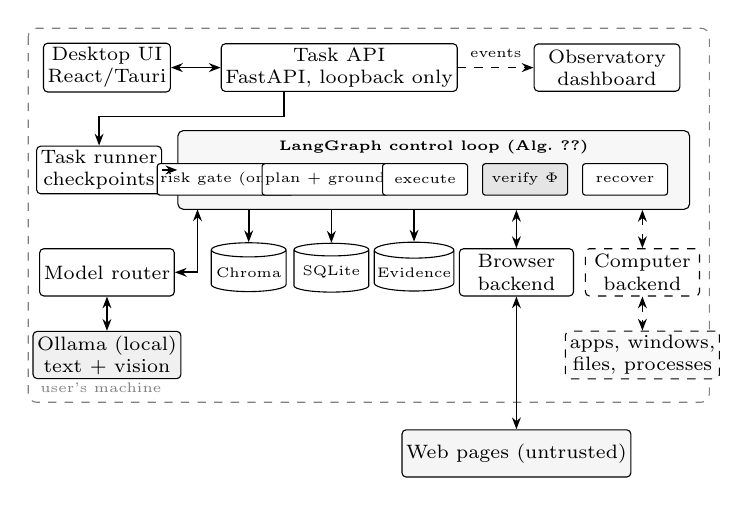
\begin{tikzpicture}[
  font=\scriptsize,
  box/.style={draw, rounded corners=1.5pt, align=center, minimum height=0.6cm, inner sep=1.5pt, fill=white},
  prop/.style={box, dashed, fill=white},
  sub/.style={draw, rounded corners=1pt, align=center, minimum height=0.4cm, minimum width=1.08cm, inner sep=1pt, font=\tiny, fill=white},
  store/.style={draw, cylinder, shape border rotate=90, aspect=0.2, align=center, minimum height=0.62cm, minimum width=0.95cm, inner sep=1pt, fill=white, font=\tiny},
  arr/.style={-{Stealth[length=1.5mm]}, semithick},
  darr/.style={{Stealth[length=1.5mm]}-{Stealth[length=1.5mm]}, semithick}]

% machine boundary
\draw[dashed, rounded corners=3pt, gray] (-0.05,0.5) rectangle (8.6,-4.25);
\node[font=\tiny, gray, anchor=south west] at (-0.02,-4.25) {user's machine};

% row 1
\node[box, minimum width=1.6cm] (ui)  at (0.95, 0) {Desktop UI\\React/Tauri};
\node[box, minimum width=2.2cm] (api) at (3.9, 0)  {Task API\\FastAPI, loopback only};
\node[box, minimum width=1.85cm] (obs) at (7.3, 0) {Observatory\\dashboard};

% row 2: runner + control loop
\node[box, minimum width=1.4cm] (run) at (0.85,-1.3) {Task runner\\checkpoints};
\node[draw, rounded corners=2pt, minimum width=6.5cm, minimum height=1.0cm, fill=gray!6] (agent) at (5.1,-1.3) {};
\node[font=\tiny\bfseries, anchor=north] at (agent.north) {LangGraph control loop (Alg.~\ref{alg:loop})};
\node[sub] (s1) at (2.45,-1.42) {risk gate (once)};
\node[sub] (s2) at (3.72,-1.42) {plan + ground};
\node[sub] (s3) at (4.99,-1.42) {execute};
\node[sub, fill=gray!20] (s4) at (6.26,-1.42) {verify $\Phi$};
\node[sub] (s5) at (7.53,-1.42) {recover};

% row 3
\node[box, minimum width=1.5cm] (router) at (0.95,-2.6) {Model router};
\node[store] (chroma) at (2.75,-2.6) {Chroma};
\node[store] (db)  at (3.8,-2.6) {SQLite};
\node[store] (ev)  at (4.85,-2.6)  {Evidence};
\node[box, minimum width=1.45cm] (bb) at (6.15,-2.6) {Browser\\backend};
\node[prop, minimum width=1.45cm] (cb) at (7.75,-2.6) {Computer\\backend};

% row 4
\node[box, minimum width=1.5cm, fill=gray!12] (oll) at (0.95,-3.65) {Ollama (local)\\text + vision};
\node[prop, minimum width=1.45cm, fill=gray!5] (loc) at (7.75,-3.65) {apps, windows,\\files, processes};

% outside
\node[box, minimum width=1.6cm, fill=gray!8] (web) at (6.15,-4.9) {Web pages (untrusted)};

% edges
\draw[darr] (ui) -- (api);
\draw[arr] ($(api.south)+(-0.7,0)$) |- (0.85,-0.62) -- (run.north);
\draw[arr] (run) -- (agent);
\draw[darr] (2.1,-1.8) |- (router.east);
\draw[darr] (router) -- (oll);
\draw[arr] (chroma.north |- agent.south) -- (chroma.north);
\draw[arr] (db.north |- agent.south) -- (db.north);
\draw[arr] (ev.north |- agent.south) -- (ev.north);
\draw[darr] (bb.north |- agent.south) -- (bb.north);
\draw[darr, dashed] (cb.north |- agent.south) -- (cb.north);
\draw[darr] (bb) -- (web);
\draw[darr, dashed] (cb) -- (loc);
\draw[arr, dashed] (api) -- node[font=\tiny, above] {events} (obs);
\end{tikzpicture}
\caption{Components of Agentic Pilot. Solid: implemented; dashed: proposed. Everything inside the boundary runs on the user's machine; the model endpoint must be a loopback address unless the user overrides it. The browser backend is the only implemented execution environment; the computer backend and the local resources it would act on are a design. The Observatory also reads the task database and evidence files.}
\label{fig:arch}
\end{figure}


Fig.~\ref{fig:arch} shows the components. A desktop client submits a task to a FastAPI service bound to the loopback interface. The control loop is a compiled LangGraph state machine with eleven nodes (Algorithm~\ref{alg:loop}); a typed state carries the intent, plan, observation, action history, counters and status. Only the verification node can end a task as \textsc{Completed}, and only when $\Phi$ holds.

\begin{algorithm}[t]
\caption{Evidence-gated control loop (browser backend)}
\label{alg:loop}
\footnotesize
\begin{algorithmic}[1]
\Require goal $g$; budget of $K{=}15$ model calls
\State $I \gets \Call{ParseIntent}{g}$; $P \gets \Call{Decompose}{g}$ if multi-step
\If{$I$ is high-risk and not approved} \Return \textsc{WaitApproval} \EndIf
\State \Call{Navigate}{$I.\mathit{site}$}; on failure go to line~\ref{alg:recover}
\Loop
  \State $o \gets \Call{Observe}{}$ \Comment{sanitized DOM, screenshot}
  \If{$\beta(o)$} \Return \textsc{Blocked} \Comment{hand off to user} \label{alg:beta}
  \EndIf
  \State $a \gets \Call{Plan}{g, P, o, \textsc{Retrieve}(g)}$ \Comment{model call}
  \State $\alpha \gets \Call{Execute}{a}$; save before/after evidence
  \If{$\alpha = 0$}
    \If{fewer than 3 retries} \textbf{continue} \EndIf
    \State $\textit{st} \gets \Call{Recover}{\text{error}}$ \label{alg:recover}
    \If{$\textit{st}$ is blocked} \Return \textsc{Blocked} \EndIf
    \If{$\textit{st}$ is exhausted} \Return \textsc{Failed} \EndIf
    \State \textbf{continue} \Comment{retry, vision, \dots}
  \EndIf
  \If{$a \neq \texttt{complete}$} mark step done; \textbf{if} steps remain \textbf{continue} \EndIf
  \If{$a = \texttt{complete}$ or last step or text typed}
    \State $(v, \text{obs}) \gets \Phi(g, s, P)$; save as evidence \label{alg:phi}
    \If{$v$} store memory; \Return \textsc{Completed} \EndIf
  \EndIf
  \If{model calls $\geq K$} go to line~\ref{alg:recover} \Comment{budget failure enters recovery} \EndIf
\EndLoop
\end{algorithmic}
\end{algorithm}


\textbf{Planning and routing.} A small model parses the request into an intent (action, site, target, content, risk); longer requests are decomposed into steps. A router assigns each call one of the installed local Qwen2.5, Qwen3.5 or DeepSeek-R1 models (1.5B--7B) or a small vision model through Ollama.

\textbf{Browser backend.} Playwright contexts over one Chromium instance give each task its own page. Each observation lists up to 50 ranked interactable elements, sanitized against prompt injection. Typed text is read back. Per task, an evidence directory holds before/after screenshots, the DOM manifest, the verification and recovery records and the node trace.

\textbf{Recovery and memory.} A failed action is retried while the task's retry counter is below three; then failures are classified into seven types and assigned a strategy (retry, alternative selector, vision fallback, replan) until the counter reaches six. Outcomes are written to a local Chroma collection and retrieved into later planning prompts.

\textbf{Locality enforcement.} The model client refuses any endpoint whose host is not a loopback address or a \texttt{localhost} name, before connecting, unless the user sets \texttt{PILOT\_ALLOW\_REMOTE\_MODEL=true}. Chroma telemetry is disabled. The backend is about 11{,}000 lines of Python, public under the MIT license; the evaluated code is commit \texttt{bf0a8a5}.

\section{Evaluation Methodology}

The evaluation comprises component-level \status{actual} experiments without a language model and a seeded \status{synthetic} simulation. Every number belongs to one evidence class: \status{actual} (measured on the implementation), \status{synthetic} (simulation output), \status{assumed}, \status{derived}, \status{literature} or \status{proposed}.

\textbf{Gate study.} A state is a goal, a URL, an HTML document served through request interception, the agent's answer and plan state, and an oracle label. The \emph{design} set (38 states) was used to find defects and design fixes; \emph{held-out~1} (12) was written after the fixes; \emph{held-out~2} (42, 22 unsatisfied) was written to a fixed procedure with varied phrasings and committed with its SHA-256 hash before the gate was run on it. Each state is judged by the predicate and by the real verification node with I/O stubbed. Paired comparisons use the exact McNemar test~\cite{mcnemar1947note}. The study ran on a 4-core 2.1\,GHz container without GPU.

\textbf{Locality test.} Ten development tasks were run under seven configurations through the real loop and Chromium against a scripted stand-in for the Ollama API on 127.0.0.1, logging every socket connection attempt of the harness's Python processes.

\textbf{Simulation.} 100 scenarios (seed 202) propagate measured detection rates and latencies through the control flow with assumed planner behaviour, chiefly the probability $\pi=0.65$ that $\Phi$ is evaluated while the task is unfinished, swept from 0.3 to 0.95; 1{,}000 Monte Carlo sets draw rates from Beta posteriors. The reported model (v2) was revised after the first model's results were known and is not pre-registered.

\section{Results}

\begin{table}[t]
\centering
\caption{Completion gate on constructed states (\status{actual}). Withheld: unsatisfied states not reported complete; FR: satisfied states rejected; $p$: exact McNemar on paired correctness}
\label{tab:gate}
\footnotesize
\setlength{\tabcolsep}{3pt}
\begin{tabular}{@{}lcccc@{}}
\toprule
Set & Withheld & FR & $p$ vs dispatch & $p$ vs $E$ only\\
\midrule
Design, before fixes & 15/23 & 3/15 & -- & --\\
Design, after fixes$^{a}$ & 20/23 & 1/15 & -- & --\\
Held-out 1 & 2/5 & 1/7 & 1.0 & 1.0\\
Held-out 2 (frozen) & 9/22 & 1/20 & 0.021 & 0.070\\
Pooled held-out & 11/27 & 2/27 & 0.022 & 0.11\\
$E$ only, held-out 2 & 2/22 & 0/20 & -- & --\\
\bottomrule
\end{tabular}

\vspace{2pt}
\raggedright\scriptsize $^{a}$No test: the fixes were designed on these states. Wilson 95\% intervals: held-out 2 withheld 0.23--0.61, FR 0.01--0.24.
\end{table}

\subsection{Completion Gate (G1)}
Table~\ref{tab:gate} reports the gate study. Before the fixes, the predicate withheld 15 of 23 unsatisfied design states, and the live node only 14 or 13, because it let a premature \texttt{complete} mark a pending step done and took the planner's reasoning for an answer. After the fixes all modes agree on every state; on design states the gate withholds 20 of 23 and rejects 1 of 15.

On held-out~2 the gate withholds 9 of 22 unsatisfied states and rejects 1 of 20 satisfied ones, correct alone on 9 states and wrong alone on 1 ($p=0.021$; pooled 11 against 2, $p=0.022$). Against a detector applying only the error check $E$, the gate is correct alone on 7 states and wrong alone on 1 ($p=0.070$): the evidence that the checks beyond $E$ add accuracy on new phrasings is suggestive but not significant. The misses follow from the rules: $X$ fires only on words such as ``extract'' and accepts any answer repeating a goal term, so none of the 5 unsatisfied extraction states is withheld; unparsed text-entry phrasings and an add-to-cart click that added nothing also pass. The one false rejection is a page that merely mentions reCAPTCHA.

\begin{table}[t]
\centering
\caption{Per-conjunct ablation (\status{actual}): false completions (of 23) and false rejections (of 15) on the design states when one check is removed}
\label{tab:abl}
\footnotesize
\setlength{\tabcolsep}{3.2pt}
\begin{tabular}{@{}lcccccccc@{}}
\toprule
 & Full & $-E$ & $-H$ & $-Q$ & $-T$ & $-X$ & $-R$ & $-\beta$\\
\midrule
FC & 3 & 8 & 7 & 4 & 6 & 6 & 4 & 5\\
FR & 1 & 1 & 1 & 1 & 1 & 0 & 1 & 1\\
\bottomrule
\end{tabular}
\end{table}

\subsection{Contribution of Each Conjunct (G2)}
Removing one conjunct at a time (Table~\ref{tab:abl}) raises false completions on the design states from 3 to 8 ($E$), 7 ($H$), 6 ($T$, $X$), 5 ($\beta$) and 4 ($Q$, $R$), but changes at most three held-out decisions, and removing $Q$ or $X$ changes none. Coverage, more than the strength of any single check, limits the gate. With at most five discordant states the smallest attainable $p$ is 0.063, so the ablation is descriptive.

\subsection{Overhead}
$\Phi$ makes no model call. Over 83 decisions the median latency was 26.8\,ms (90th percentile 29.5, 95th 30.3, maximum 34.6\,ms); on self-hosted pages $\Phi$ alone took 5.2\,ms against 61\,ms for a screenshot and 76\,ms for DOM extraction.

\subsection{Locality (G3), Memory, Recovery and Oracle}
In 70 episodes, all 555 connection attempts of the agent's eight Python processes went to the stand-in on 127.0.0.1, and every page request named 127.0.0.1; a rerun on a clean commit gave the same result. UDP, DNS, Chromium and the model server were not instrumented. Memory retrieval on 10 queries over 22 records gave P@3 0.52 (the attainable maximum), R@3 1.00 and MRR 0.93, but the top record was irrelevant or retrieval failed in 3 of 10 queries, since retrieval has no relevance threshold. The recovery engine classified a missing confirmation as \emph{unknown} and assigned the generic sequence. The end-to-end oracle agreed with the intended verdict on all 114 scripted trajectories (0 false negatives on 35 solutions, 0 false positives on 34 near misses), and 144 of 147 tests pass.

\begin{table}[t]
\centering
\caption{Simulation summary (\status{synthetic}, v2, post hoc; conditional on \status{assumed} planner behaviour)}
\label{tab:sim}
\footnotesize
\setlength{\tabcolsep}{3pt}
\begin{tabular}{@{}p{0.6cm}p{3.3cm}p{3.9cm}@{}}
\toprule
Hyp. & Quantity & Result\\
\midrule
H1 & False completions (100 scenarios) & 19 with $\Phi$ vs 28 none; $-0.11$ per scenario [0.05, 0.18]\\
H2 & Correct decisions (74 claims) & 52 vs 46 accept-all; $p=0.15$\\
-- & Tasks achieved and reported & 44 with $\Phi$ vs 46 none\\
H3 & Repeated workflows (of 44) & 19 / 19 / 20 (none / memory / proposed filter)\\
H4 & Failures recovered (of 93) & 51 / 68 / 87 (retries / engine / proposed)\\
H5 & Mean episode time & $+2.6\%$ with $\Phi$; $+14\%$ self-check\\
\bottomrule
\end{tabular}
\end{table}

\subsection{Simulation (\status{synthetic})}
Table~\ref{tab:sim} summarizes the simulation. Values here follow from measured component behaviour and \status{assumed} planner behaviour and are not measurements of the agent. Episodes end in a false completion 19 times with $\Phi$ against 28 without verification, a paired reduction of 0.11 per scenario [0.05, 0.18]; the direction is fixed by construction. On 74 claims, $\Phi$ decides correctly in 52 and accept-all in 46 ($p=0.15$; better at $p<0.05$ in 42\% of Monte Carlo sets), so H2 is not supported. Repeated workflows succeed 19 times of 44 with and without memory, which is too few to detect the assumed effect; the recovery engine recovers 68 of 93 recoverable failures against 51 for inline retries alone, and the proposed evidence-guided variant reaches 87 only by assumption. Two of $\Phi$'s three false rejections come from an assumed missing-evidence rejection rate of 0.8, whereas the measured rate is 0 of 24. $\Phi$ lengthens the mean episode by 2.6\%, a model self-check by 14\%. As $\pi$ rises from 0.3 to 0.95, FCR rises from 0.14 to 0.32 with $\Phi$ and from 0.21 to 0.45 without verification, while FRR stays near 0.14 against 0.08.

\section{Safety, Privacy and Autonomy}

\textbf{Threat model.} The user and the host are trusted; content the agent reads is not. We consider injected instructions~\cite{greshake2023indirect}, high-impact actions without consent, exposure of credentials and sensitive screenshots, and disclosure of user data to a model provider; a compromised host, browser or model is out of scope.

\textbf{Privacy property.} By default the model client sends prompts and screenshots only to a model server on the loopback interface, and the code writes task records, memory and evidence only to local files. Evidence for it is the endpoint refusal, disabled Chroma telemetry and the egress test. It does not cover what the loopback model server does with a request, data entered on websites, one-time downloads of model weights, or proxy environment variables. It is a property of data locality under the default configuration, not a formal privacy guarantee.

\textbf{Autonomy.} The agent acts only in the browser and exposes no file, process or command action. A task classified as posting, e-mailing, purchasing, deleting or transferring waits for the user's approval; bot checks stop the task for the user; a sanitizer replaces 17 injection patterns in element text; the service listens only on loopback. The sanitizer is a fixed denylist, the approval decision is made once per task by a small model, and the local API has no authentication, so security hardening remains future work.

\section{Discussion and Limitations}

A rule over the observed page is a cheap and inspectable way to withhold premature completions, and storing the inputs of each decision exposed real defects. Its rules, however, generalize only partly: 20 of 23 on design states fell to 9 of 22 on frozen held-out states. Hand-written rules are keyed to the wording they were written for; model-based judges~\cite{pan2024autonomous,sumyk2025done} cover broader goals but add inference cost and are models judging models~\cite{huang2024cannot}, so the two are likely complementary. Typed answer checks, wider trigger vocabularies and a measured model judge for requests that no rule covers are natural extensions; memory needs a relevance threshold and recovery a missing-confirmation class.

The states are constructed, and their labels were written by the AI assistant that also designed the fixes, without a second annotator. The sets are small. The egress test used a stand-in model server and covered the Python processes only. The simulation is post hoc and conditional on assumed planner behaviour. Task-level success of the full agent with a language-model planner is outside the scope of this study; a 40-task harness on five self-hosted sites, with a validated oracle, is released for it.

\section{Conclusion}

Agentic Pilot separates action dispatch from task completion and keeps model traffic on the user's machine. On frozen held-out states its completion gate withheld 41\% of premature completions with one false rejection in 20, beating a dispatch-only rule at a cost of 27\,ms per decision, and its Python processes contacted only the loopback interface. The claims are confined to the evaluated components and the stated simulation conditions.

\section*{Acknowledgment}
The authors thank the Department of Computing Technologies, SRM Institute of Science and Technology. Code and data: \url{https://github.com/sudeshsudhii/Agentic-pilot-local}.

\bibliographystyle{IEEEtran}
\bibliography{references}

\end{document}
